\documentclass{article}
\usepackage{graphicx} 
\usepackage[colorlinks=true, linkcolor=blue, urlcolor=red]{hyperref}
\usepackage[utf8]{inputenc}
\usepackage[T1]{fontenc}
\usepackage{lmodern} 
\usepackage[polish]{babel}
\usepackage{float} 
\usepackage{listings}
\usepackage{xcolor}

\lstnewenvironment{Rcode}[1][]{
    \lstset{
        language=R,
        basicstyle=\ttfamily,
        keywordstyle=\color{blue},
        commentstyle=\color{green!40!black},
        stringstyle=\color{orange},
        showstringspaces=false,
        frame=single,
        numbers=left,
        numberstyle=\tiny,
        numbersep=5pt,
        breaklines=true,
        #1
    }
}{}

\title{Statystyka Wielowymiarowa}
\author{Adam Staniszewski}
\date{May 2024}

\begin{document}

\maketitle

\tableofcontents  % Add table of contents here

\section{Dobór zbioru danych}
Do wykonywania zadań został wybrany zbiór \href{https://www.kaggle.com/datasets/girumwondemagegn/dataset-for-renewable-energy-systems}{Dataset for renewable energy systems}. Składa się on z 13 kolumn i około 15000 wierszy. 

Dodatkowo, dla zadań klasyfikacji binarnej, kolumna \textbf{Type\_of\_Renewable\_Energy} została przerobiona na 7 osobnych kolumn, reprezentujących źródła energii:
\begin{itemize}
    \item \textbf{Solar},
    \item \textbf{Wind},
    \item \textbf{Hydroelectric},
    \item \textbf{Geothermal},
    \item \textbf{Biomass},
    \item \textbf{Tidal},
    \item \textbf{Wave},
\end{itemize}

\section{Laboratorium 1}
\subsection{Regresja liniowa}
Na początku przeprowadzamy prostą regresję liniową:

\begin{figure}[H]
    \centering
    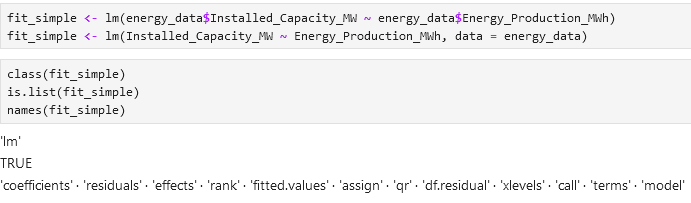
\includegraphics[width=0.9\linewidth]{lab1/obraz.png}
    \caption{Zmienna objaśniana - Installed Capacity MW. Zmienna objaśniająca - Energy Production MWh}
    \label{fig:regression}
\end{figure}

\begin{figure}[H]
    \centering
    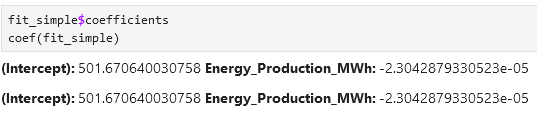
\includegraphics[width=0.9\linewidth]{lab1/obraz2.png}
    \caption{Współczynniki regresji}
    \label{fig:coefficients}
\end{figure}

\begin{figure}[H]
    \centering
    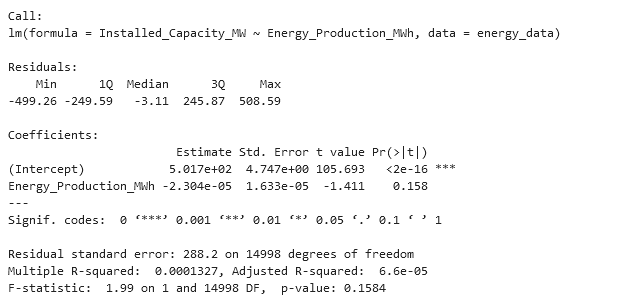
\includegraphics[width=0.9\linewidth]{lab1/obraz3.png}
    \caption{Podsumowanie regresji liniowej}
    \label{fig:summary}
\end{figure}

\begin{figure}[H]
    \centering
    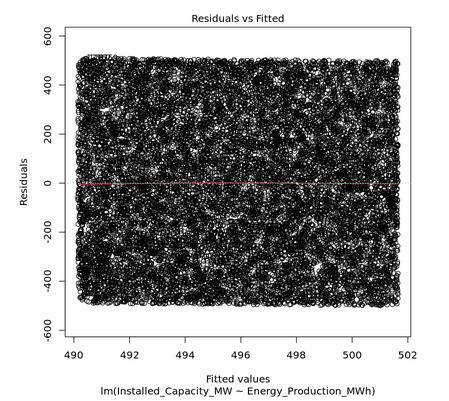
\includegraphics[width=0.9\linewidth]{lab1/obraz4.png}
    \caption{Wartości rzeczywiste vs przewidywane}
    \label{fig:real_vs_predicted}
\end{figure}

\begin{figure}[H]
    \centering
    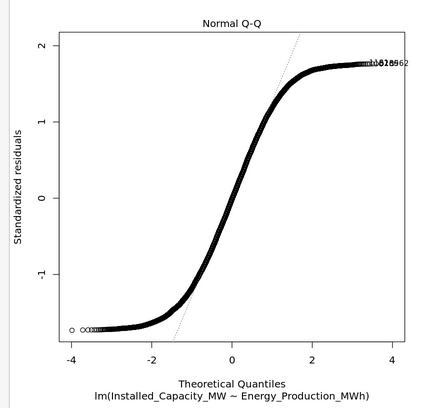
\includegraphics[width=0.9\linewidth]{lab1/obraz5.png}
    \caption{Reszty regresji}
    \label{fig:residuals}
\end{figure}

\begin{figure}[H]
    \centering
    \includegraphics[width=0.9\linewidth]{lab1/obraz6.png}
    \caption{Heat values}
    \label{fig:heat_values}
\end{figure}

\subsection{Regresja wielokrotna}
Przejdźmy do regresji wielokrotnej. Będziemy przewidywać wartość \textbf{Installed\_Capacity\_MW} na podstawie zmiennych \textbf{Energy\_Production\_MWh} i \textbf{Energy\_Consumption\_MWh}.

\begin{Rcode}
fit_la <- lm(energy_data$Installed_Capacity_MW ~ energy_data$Energy_Production_MWh + energy_data$Energy_Consumption_MWh)
\end{Rcode}

\begin{figure}[H]
    \centering
    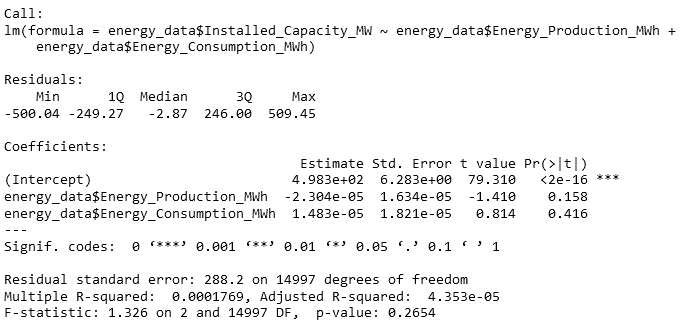
\includegraphics[width=1\linewidth]{lab1/obraz9.png}
    \caption{Enter Caption}
    \label{fig:enter-label}
\end{figure}

Przeprowadźmy teraz regresję wielokrotną dla jednej zmiennej dla pozostałych zmiennych liczbowych:

\begin{Rcode}
numerical_data <- energy_data[, sapply(energy_data, is.numeric)]
fit_all <- lm(Installed_Capacity_MW ~ ., data = numerical_data)
\end{Rcode}

\begin{figure}[H]
    \centering
    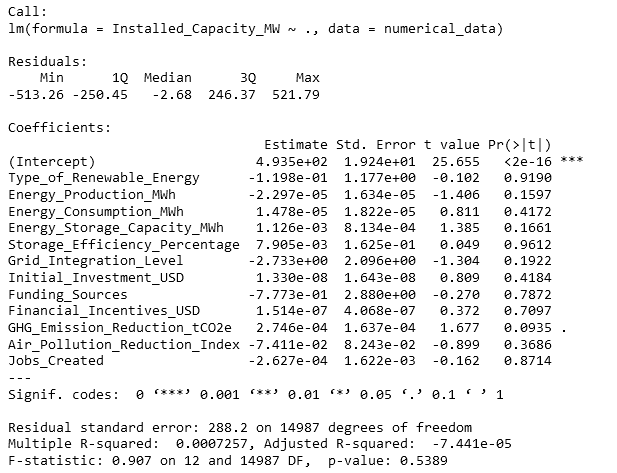
\includegraphics[width=1\linewidth]{lab1/obraz10.png}
    \caption{Enter Caption}
    \label{fig:enter-label}
\end{figure}

\begin{figure}[H]
    \centering
    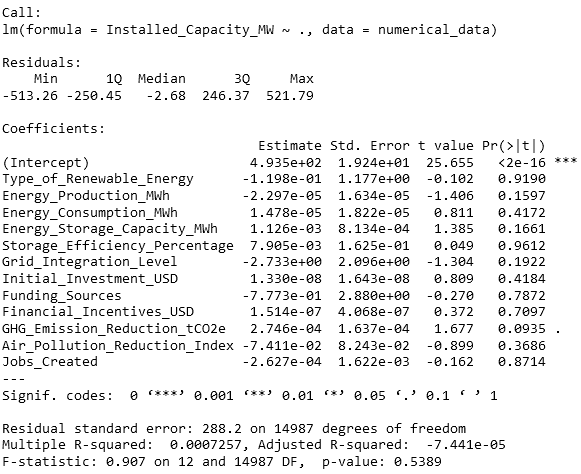
\includegraphics[width=1\linewidth]{lab1/obraz11.png}
    \caption{Enter Caption}
    \label{fig:enter-label}
\end{figure}

A teraz bez zmiennej Grid\_Integration\_Level:

\begin{Rcode}
fit_no_grid_int <- update(fit_all, ~ . - Grid_Integration_Level)
summary(fit_no_grid_int)
\end{Rcode}

\begin{figure}[H]
    \centering
    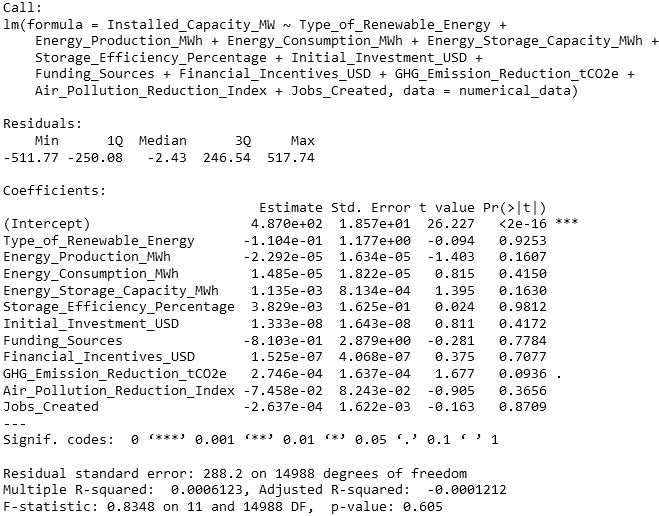
\includegraphics[width=1\linewidth]{lab1/obraz12.png}
    \caption{Enter Caption}
    \label{fig:enter-label}
\end{figure}

Wybrane przedziały ufności:

\begin{figure}[H]
    \centering
    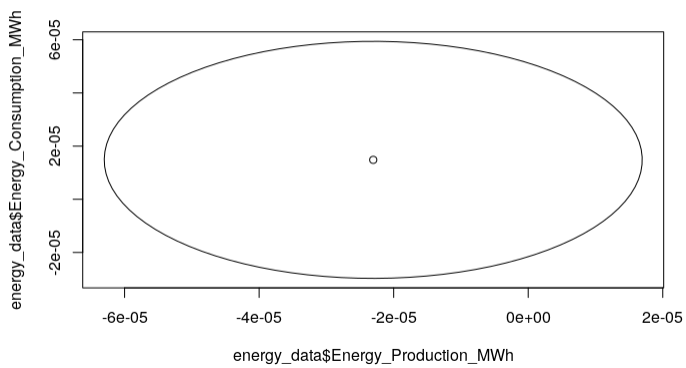
\includegraphics[width=1\linewidth]{lab1/obraz13.png}
    \caption{Enter Caption}
    \label{fig:enter-label}
\end{figure}

Sprawdźmy jeszcze jak poradzi sobie regresja wielomianowa (5 stopnia):

\begin{Rcode}
anova(fit_simple, fit_l2)
fit_l5 <- lm(energy_data$Energy_Consumption_MWh ~ poly(energy_data$Energy_Production_MWh, 5))
summary(fit_l5)
summary(lm(Energy_Production_MWh ~ log(Energy_Consumption_MWh), data = energy_data))
\end{Rcode}

\begin{figure}[H]
    \centering
    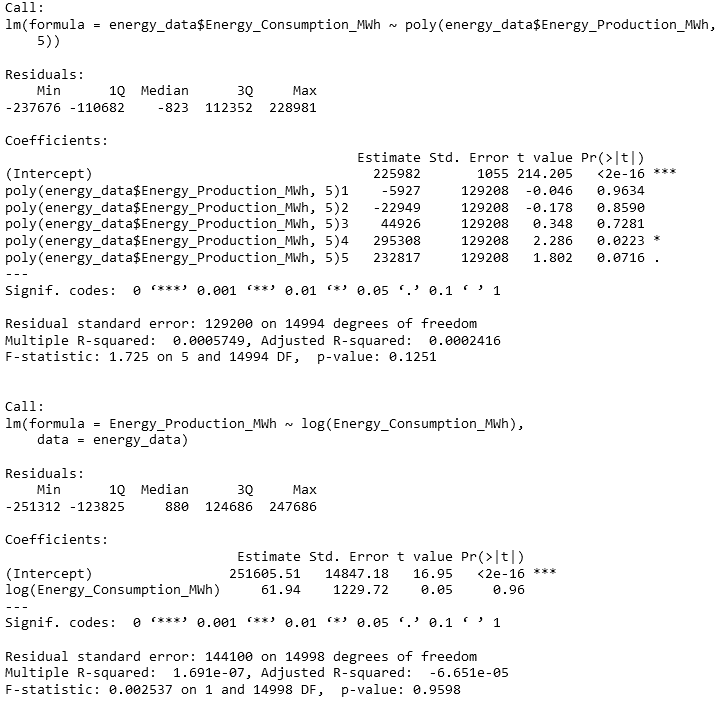
\includegraphics[width=1\linewidth]{lab1/obraz14.png}
    \caption{Enter Caption}
    \label{fig:enter-label}
\end{figure}

\section{Laboratorium 2}
\subsection{One hot encoding i korelacje}
Jak wspomniano we wstępie, dla zadań klayfikacji binarnej wykonany został \textbf{One Hot Encoding} kolumny \textbf{Type\_Of\_Renewable\_Energy}. Ze względu na problemy ze środowiskiem wykonawczym, odpowiednia funkcja została napisana bez użycia zewnętrznych bibliotek:

\begin{Rcode}
unique_types <- unique(energy_data$Type_of_Renewable_Energy)

for (type in unique_types) {
  column_name <- paste("Type_of_Renewable_Energy", type, sep = "_")
  energy_data[[column_name]] <- ifelse(energy_data$Type_of_Renewable_Energy == type, 1, 0)
}

energy_data <- subset(energy_data, select = -c(Type_of_Renewable_Energy))
\end{Rcode}

Otrzymujemy w ten sposób 7 dodatkowych kolumn o binarnych wartościach, które zostaną użyte jako cel klasyfikacji.

Znajdźmy najsilniejsze korelacje między cechami (pomijając korelacje między tymi samymi cechami):

\begin{Rcode}
numeric_data <- energy_data[sapply(energy_data, is.numeric)]
corr_mat <- cor(numeric_data)
corr_df <- as.data.frame(as.table(corr_mat))
corr_df <- corr_df[corr_df$Var1 != corr_df$Var2,]
corr_df <- corr_df[order(abs(corr_df$Freq)),]
top_corrs <- head(corr_df, 10)
\end{Rcode}

\begin{figure}[H]
    \centering
    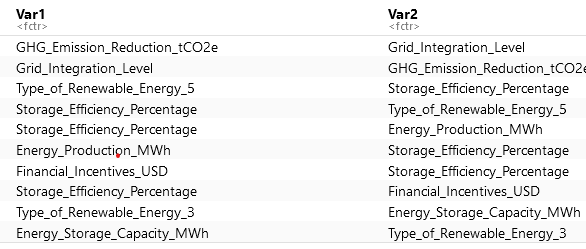
\includegraphics[width=1\linewidth]{lab2/obraz.png}
    \caption{Zmienne o najwyższych korelacjach.}
    \label{fig:enter-label}
\end{figure}

\subsection{Regresja logistyczna}

Spróbujmy przywidzieć czy dane źródło energii należy do \textbf{1 kategorii} za pomocą zmiennych \textbf{Installed\_Capacity\_MW}, \textbf{Energy\_Production\_MWh}, \textbf{Energy\_Storage\_Capacity\_MWh} i \textbf{Storage\_Efficiency\_Percentage}.

\begin{Rcode}
dir_logistic <- list()
dir_logistic$fit <- glm(Type_of_Renewable_Energy_1 ~ Installed_Capacity_MW + Energy_Production_MWh 
                        + Energy_Storage_Capacity_MWh + Storage_Efficiency_Percentage, 
                   family = binomial, data = energy_data)
dir_logistic$predicted <- ifelse(dir_logistic$probs > 0.5, "Type 1", "Not type 1")
dir_logistic$cm <- table(dir_logistic$predicted, energy_data$Type_of_Renewable_Energy_1)
dir_logistic$cm
\end{Rcode}

Otrzymujemy wyniki:
\begin{figure}[H]
    \centering
    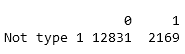
\includegraphics[width=0.7\linewidth]{lab2/obraz3.png}
    \caption{Nienależność i należność do badanej klasy}
    \label{fig:enter-label}
\end{figure}

Finalnie otrzymaliśmy proporcję błędów treningowych równą 0 - być może zadanie jest zbyt trywialne. Sprawdźmy jak wyniki zmieni poprawny podział zbioru.

\subsection{Podział zbioru}
Losowo dzielimy zbiór na treningowy i testowy w proporcjach 70/30:

\begin{Rcode}
set.seed(123)

train_indices <- sample(nrow(energy_data), round(0.7 * nrow(energy_data)))
train <- energy_data[train_indices, ]
energy_data_test <- energy_data[-train_indices, ]
Type_of_Renewable_Energy_1_test <- energy_data_test$Type_of_Renewable_Energy_1
\end{Rcode}

Wykonujemy regresję na zbiorze treningowym:

\begin{Rcode}
dir_log_t <- list()
dir_log_t$fit <- glm(Type_of_Renewable_Energy_1 ~ Installed_Capacity_MW + Energy_Production_MWh, 
                   family = binomial, data = train)
\end{Rcode}

\begin{figure}[H]
    \centering
    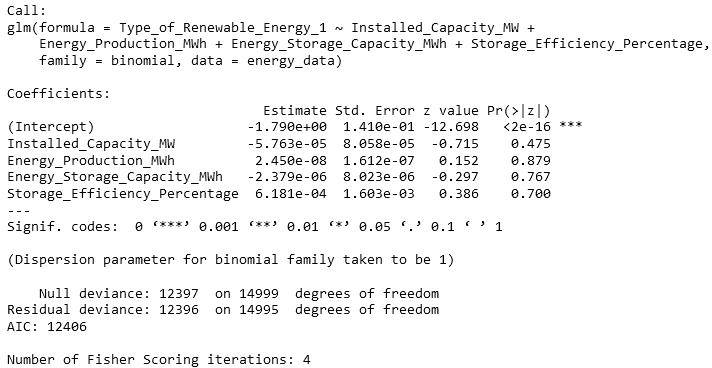
\includegraphics[width=1\linewidth]{lab2/obraz4.png}
    \caption{Podsumowanie regresji na zbiorze treningowym.}
    \label{fig:enter-label}
\end{figure}

Sprawdźmy predykcje na zbiorze testowym:

\begin{Rcode}
dir_log_t$probs <- predict(dir_log_t$fit, energy_data_test, type = "response")
dir_log_t$predicted <- ifelse(dir_log_t$probs > 0.5, "Type 1", "Not type 1")
table(dir_log_t$predicted, Type_of_Renewable_Energy_1_test)
\end{Rcode}

\begin{figure}[H]
    \centering
    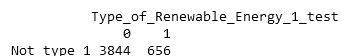
\includegraphics[width=0.75\linewidth]{lab2/obraz5.png}
    \caption{Macierz pomyłek}
    \label{fig:enter-label}
\end{figure}

W tym przypadku otrzymaliśmy proprocję błędów na poziomie około 20\%.

Użyjmy predyktorów mocniej skorelowanych ze zmienną objaśnianą, czyli \textbf{Energy\_Production\_MWh} i \textbf{Energy\_Storage\_Capacity\_MWh}:

\begin{Rcode}
dir_log_best2$fit <- glm(Type_of_Renewable_Energy_1 ~ Installed_Capacity_MW + Energy_Production_MWh, 
                         family = binomial, 
                    data = energy_data, subset = train)
summary(dir_log_best2$fit)
dir_log_best2$probs <- predict(dir_log_best2$fit, energy_data_test, type = "response")
dir_log_best2$predicted <- ifelse(dir_log_best2$probs > 0.5, "Type 1", "Not type 1")
table(dir_log_best2$predicted, Type_of_Renewable_Energy_1_test)
\end{Rcode}

\subsection{Metoda LDA}
Dokonajmy ponownego podziału na potrzeby kolejnych metod klasyfikacji:
\begin{Rcode}
set.seed(123) 
train_indices <- sample(1:nrow(energy_data), 0.7 * nrow(energy_data))
train <- rep(FALSE, nrow(energy_data))
train[train_indices] <- TRUE

test <- !train
test <- energy_data[test, ]
\end{Rcode}

Przeprowadzamy \textbf{LDA} wraz z obliczeniem proporcji błędów na zbiorze testowym:
\begin{Rcode}
dir_lda <- list()
dir_lda$fit <- lda(Type_of_Renewable_Energy_1 ~ Energy_Production_MWh + Energy_Storage_Capacity_MWh, data = energy_data, subset = train)

print(dir_lda$fit)

dir_lda$predicted <- predict(dir_lda$fit, test)
predicted_classes <- dir_lda$predicted$class
actual_classes <- test$Type_of_Renewable_Energy_1
num_errors <- sum(predicted_classes != actual_classes)

total_samples <- length(actual_classes)
proportion_of_errors <- num_errors / total_samples

print(proportion_of_errors)
\end{Rcode}

Podsumowanie LDA:
\begin{figure}[H]
    \centering
    \includegraphics[width=1\linewidth]{lab2/obraz6.png}
    \caption{Podsumowanie LDA}
    \label{fig:enter-label}
\end{figure}

Prawdopodobieństwo przynależności do klasy wynosi około 14.4\%. Jeśli weźmiemy pod uwagę, że mamy 7 możliwych klas, to będziemy w stanie wywnioskować, że zbiór jest zbalansowany pod względem ich liczności.

Proporcja błędu to z kolei około 14.6\% - lepiej niż przy regresji logistycznej.

\subsection{Metoda QDA}
Przeprowadźmy analogiczną analizę przy pomocy \textbf{QDA}:

\begin{Rcode}
dir_qda <- list()
dir_qda$fit <- qda(Type_of_Renewable_Energy_1 ~ Energy_Production_MWh + Energy_Storage_Capacity_MWh, data = energy_data, subset = train)

print(dir_qda$fit)

dir_qda$predicted <- predict(dir_qda$fit, test)
predicted_classes <- dir_qda$predicted$class

actual_classes <- test$Type_of_Renewable_Energy_1
num_errors <- sum(predicted_classes != actual_classes)
total_samples <- length(actual_classes)

proportion_of_errors <- num_errors / total_samples
print(proportion_of_errors)
\end{Rcode}

\begin{figure}[H]
    \centering
    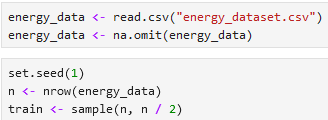
\includegraphics[width=1\linewidth]{lab2/obraz7.png}
    \caption{Podsumowanie QDA}
    \label{fig:enter-label}
\end{figure}

Proporcja błędów jest w tym przypadku taka sama, jak w LDA.

\subsection{Metoda kNN}
Na koniec sprawdźmy wyniki dla metody \textbf{kNN}, dla różnych wartości parametru \textbf{k}. W tym przypadku lekko modyfikujemy zbiory:

\begin{Rcode}
train_set <- energy_data[train, c("Energy_Storage_Capacity_MWh", "Energy_Production_MWh")]
test_set <- energy_data[!train, c("Energy_Storage_Capacity_MWh", "Energy_Production_MWh")]
renewable_energy_train <- energy_data$Type_of_Renewable_Energy_1[train]
Type_of_Renewable_Energy_1_test <- energy_data$Type_of_Renewable_Energy_1[!train]  
\end{Rcode}

Używamy kNN w pętli:
\begin{Rcode}
dir_knn <- knn(train_set, test_set, renewable_energy_train, k = k)
num_errors <- sum(dir_knn != Type_of_Renewable_Energy_1_test)
total_samples <- length(Type_of_Renewable_Energy_1_test)
\end{Rcode}

Zależność proporcji błędu od ilości parametrów:

\begin{figure}[H]
    \centering
    \includegraphics[width=1\linewidth]{lab2/obraz8.png}
    \caption{Wyniki dla kNN}
    \label{fig:enter-label}
\end{figure}

Dla \( k \geq 2 \) widzimy wartości wyższe lub zbliżone do regresji logistycznej. Dla wartości \( k \leq 8 \) wartości są najlepsze ze wszystkich metod.



\section{Laboratorium 3}
\subsection{Walidacja krzyżowa}
\subsubsection{Metoda zbioru walidacyjnego}
Na początku wczytuję dane, usuwam wartości NaN i przygotowuję zbiór walidacyjny.

\begin{Rcode}
energy_data <- read.csv("energy_dataset.csv")
energy_data <- na.omit(energy_data)
set.seed(1)
n <- nrow(energy_data)
train <- sample(n, n / 2)
\end{Rcode}
Dopasowuję model liniowy na zbiorze uczącym i obliczam MSE dla zbioru walidacyjnego:

\begin{Rcode}
energy_lm <- lm(Type_of_Renewable_Energy ~ Energy_Production_MWh,
                 data = energy_data,
                 subset = train)

validation_set <- energy_data[-train,]

mse <- mean((validation_set$Type_of_Renewable_Energy -
              predict(energy_lm, validation_set))^2)

\end{Rcode}
Otrzymana wartość MSE: \textbf{4.0439057662439}.

Użyjmy wielomianów o różnych stopniach:

\end{Rcode}
Dopasowuję model liniowy na zbiorze uczącym i obliczam MSE dla zbioru walidacyjnego:

\begin{Rcode}
for (i in 2:5) {
  energy_lm_poly <- lm(Type_of_Renewable_Energy ~ poly(Energy_Production_MWh, degree = i), data = energy_data, 
                     subset = train)
  print(mean((validation_set$Type_of_Renewable_Energy - predict(energy_lm_poly, validation_set))^2))
}
\end{Rcode}
Otrzymujemy MSE: 

\begin{Rcode}
[1] 4.042959
[1] 4.041494
[1] 4.041374
[1] 4.042979
\end{Rcode}
\textbf{Wniosek} - stopień wielomianu w tym przypadku nie ma znaczącego wpływu na otrzymany MSE.
Powtarzam obliczenia dla innego zbioru walidacyjnego:

\begin{Rcode}
degree_max <- 5

compute_mse <- function(degree, train) {
  energy_lm <- lm(Type_of_Renewable_Energy ~ poly(Energy_Production_MWh, degree), data = energy_data, subset = train)
  validation_set <- energy_data[-train,]
  mean((validation_set$Type_of_Renewable_Energy - predict(energy_lm, validation_set))^2)
}

mse <- vapply(1:degree_max, compute_mse, FUN.VALUE = numeric(1), train = train)
\end{Rcode}
Otrzymane wartości MSE:
\begin{Rcode}
4.04390576624393
4.04295881295649
4.04149420436449
4.04137383913034
4.04297885010734
\end{Rcode}

\begin{figure}[H]
    \centering
    \includegraphics[width=0.8\linewidth]{lab1/obraz8.png}
    \caption{Zależność między wartością MSE a stopniem wielomianu.}
    \label{fig:enter-label}
\end{figure}

\subsubsection{Walidacja krzyżowa bez jednego (leave-one-out)}

\begin{Rcode}
compute_loocv_mse <- function(degree) {
  energy_glm <- glm(Type_of_Renewable_Energy ~ poly(Energy_Production_MWh, degree), data = energy_data)
  cv.glm(energy_data, energy_glm)$delta[1]
}
mse <- sapply(1:degree_max, compute_loocv_mse)
mse
\end{Rcode}

\begin{Rcode}
    TUTAJ WYKRES TEGO WYZEJ
\end{Rcode}

\begin{Rcode}
[Co teraz z wnioskami na temat regresji wielomianowej w naszym przypadku?]
[Sprawdź, że dla LOOCV obie współrzędne delta zawierają praktycznie to samo.]
\end{Rcode}

\subsubsection{K-krotna walidacja krzyżowa}
Tym razem jawnie ustawiamy parametr K oznaczający liczbę grup:

\begin{Rcode}
compute_kcv_mse <- function(degree, k) {
    energy_glm <- glm(Type_of_Renewable_Energy ~ poly(Energy_Production_MWh, degree), data = energy_data)
    cv.glm(energy_data, energy_glm, K = k)$delta[1]
}
mse <- sapply(1:degree_max, compute_kcv_mse, k = 10)
\end{Rcode}
Zestawiamy 10 wyników:
\begin{Rcode}
mse10 <- replicate(10, sapply(1:degree_max, compute_kcv_mse, k = 10))
\end{Rcode}
Otrzymujemy:
\begin{Rcode}
    10 WYNIKOW
\end{Rcode}
\begin{Rcode}
    WYKRES
\end{Rcode}
\begin{Rcode}
    CO Z WYNIKAMI
\end{Rcode}

\subsubsection{Bootstrap}
\begin{Rcode}

}
\end{Rcode}

\subsection{Selekcja cech dla modeli liniowych}
\subsubsection{Selekcja krokowa do przodu i wstecz}
\subsubsection{Wybór modelu przy pomocy metody zbioru walidacyjnego}
\subsubsection{Wybór modelu przy pomocy k-krotnej walidacji krzyżowej}

\section{Laboratorium 4}
\subsection{Regularyzacja}
\subsubsection{Regresja grzbietowa}
\subsubsection{Lasso}
\subsection{Modele nieliniowe}
\subsubsection{Regresja wielomianowa}
\subsubsection{Regresja logistyczna wielomianowa}
\subsubsection{Funkcje schodkowe}
\subsection{Funkcje sklejane}
\subsubsection{Naturalne funkcje sklejane}
\subsubsection{Wygładzające funkcje sklejane}
\subsection{Regresja lokalna}
\subsection{Uogólnione modele addytywne (GAMs)}
\subsection{GAM w GLM}

\end{document}
